\graphicspath{{images/}{images/logos/}}

\begin{frame}{Meine Tätigkeiten}
	\begin{itemize}
		\item Neues Bewegungsmodell für das Pferd
		\begin{itemize}
			\item Pferde Modell
			\item Schritt Optimierung generalisiert
			\item Logik für Diskretisierung der Ellipse
		\end{itemize}
	\end{itemize}
\end{frame}  


\begin{frame}{Gangart eines Pferdes}
	\begin{center}
		%\movie[label=show3,width=1.0\textwidth,poster,autostart,showcontrols,loop]{}{movies/schritt.mp4}
		%\movie[label=show3,width=1.0\textwidth,poster,autostart,showcontrols,loop]{}{movies/trap.mp4}
		%\movie[label=show3,width=1.0\textwidth,poster,autostart,showcontrols,loop]{}{movies/galopp.mp4}
		\includemovie[poster,text={\small(Loading movies/schritt.mp4)}]{6cm}{6cm}{movies/schritt.mp4}
		\includemovie[poster,text={\small(Loading movies/schritt.mp4)}]{6cm}{6cm}{movies/trap.mp4}
		\includemovie[poster,text={\small(Loading movies/schritt.mp4)}]{6cm}{6cm}{movies/galopp.mp4}
						
	\end{center}
\end{frame}

\begin{frame}{Wendigkeit eines Pferdes}
	%\begin{tabular}{cc}		
		\begin{minipage}{0.5\textwidth}
			\begin{figure}[H]
				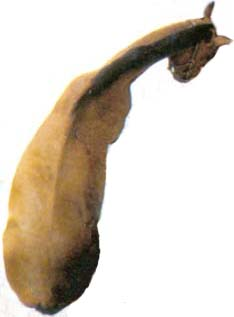
\includegraphics[width=50px, height=250px, keepaspectratio]{appendix/images/horsebend.jpg}		
				\caption{\label{fig:blue_rectangle} Rechtsschritt}
			\end{figure}
		\end{minipage} \hfill
		\begin{minipage}{0.45\textwidth}
			\begin{itemize}
				\item Ein Pferd hat nicht die selben Bewegungsfreiheiten wie ein Mensch.
				\item Wendigkeit wirkt sich auf erreichbare Positionen aus!
			\end{itemize}
			$\rightarrow$ Seitwärts Schritte sind kürzer als Gerade aus! \newline
			$\rightarrow$ Nur Bewegung nach vorne möglich!
		\end{minipage}				
	%\end{tabular}
\end{frame}

\begin{frame}{Das Model}
		\begin{minipage}{0.5\textwidth}
			\begin{figure}[H]
				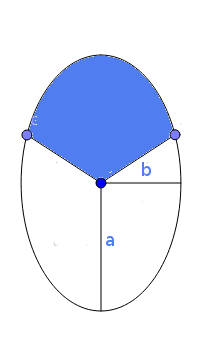
\includegraphics[width=50px, height=250px, keepaspectratio]{appendix/images/ellipse.png}		
				\caption{\label{fig:blue_rectangle} Bewegungsmuster}
			\end{figure}
		\end{minipage} \hfill
		\begin{minipage}{0.45\textwidth}
			Die Eigenschaften der Ellipse werden durch die Gangart bestimmt. 
			Eine schnelle Gangart führt zu größeren Maßen $a$ und $b$ und zu kleineren Bewegungswinkeln. \newline \newline
			$\rightarrow$ Geeignet für das Optimal Steps Model (OSM) \newline

		\end{minipage}	
\end{frame}

\begin{frame}{Stand davor}
	\begin{center}
		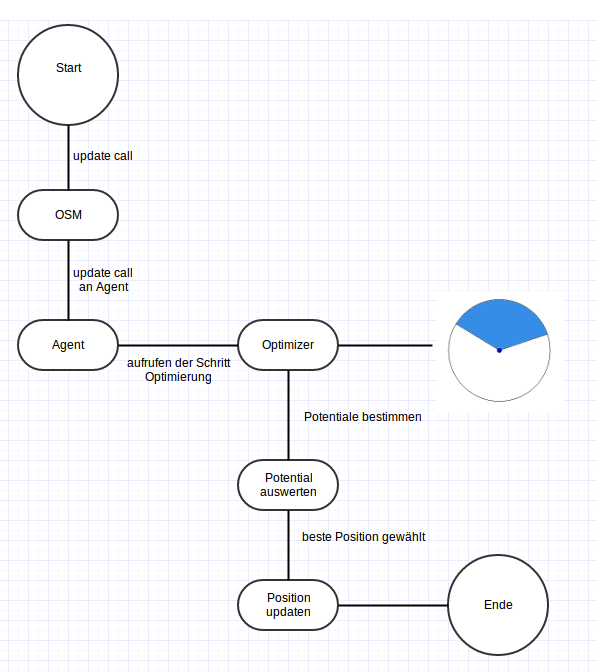
\includegraphics[width=200px, height=200px, keepaspectratio]{appendix/images/struct.png}		
	\end{center}
\end{frame}

\begin{frame}{Stand heute}
	\begin{center}
		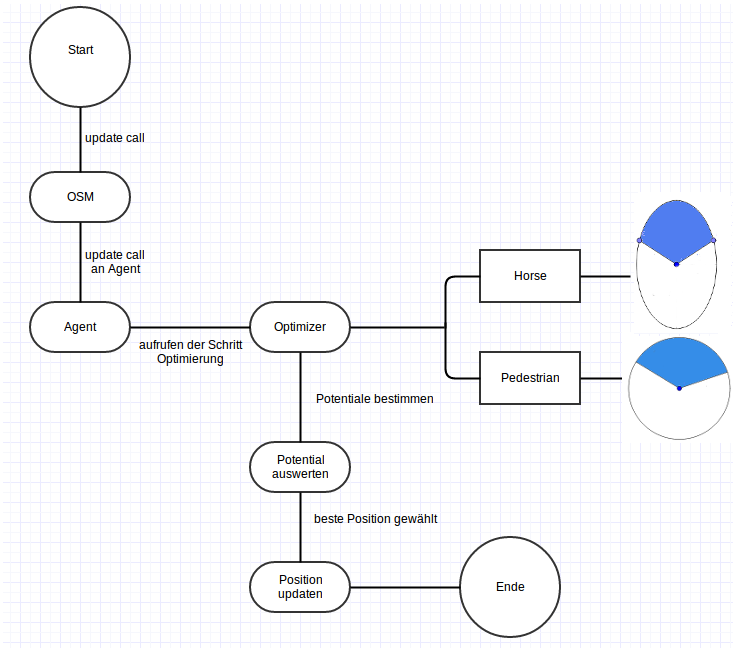
\includegraphics[width=200px, height=200px, keepaspectratio]{appendix/images/struct_new.png}		
	\end{center}	
\end{frame}

%\begin{frame}{Step Optimizer und Diskretisierung}
	% step optimizer und diskretisierung erzählen
	% nutz normale ellipse und rotiert die. Wieso kein winkel eingeführt? 
	% -> tiefgreifende veränderung + rotation für kreise nicht notwendig und würde bloß performance kosten.
%\end{frame}

\begin{frame}{Fazit}
	\begin{itemize}
		\item Fand ich gut:
			\begin{itemize}
				\item Team hält sich an Aufteilung
			\end{itemize}

		\item Kann besser sein:
			\begin{itemize}
				\item Zu wenig Einblick in Aufgaben der anderen Mitglieder
			\end{itemize}
		\item Anteil Schätzung: \tab 23\%
	\end{itemize}
\end{frame}